\documentclass{article}

\usepackage{amsmath}
\usepackage{enumitem}
\usepackage{graphicx}
\usepackage{xcolor}
\usepackage{subcaption}
\usepackage{xepersian}

\settextfont{XB Kayhan}
\setmathdigitfont{Yas}
\setlatintextfont{Times Newer Roman}

\title{\vspace{-4cm} \textbf{پاسخ تمرینات سری دوم درس شناسایی آماری الگو}}
\author{محمدرضا غفرانی  ۴۰۰۱۳۱۰۷۶}
\date{\today}

\begin{document}
\maketitle

\section*{سوال یک}

\subsection*{قسمت الف}

در ابتدا شرکت‌کننده می‌تواند هر یک از در‌ها را انتخاب کند، از آن جا که احتمال انتخاب هر یک از در‌ها با
یکدیگر برابر است در نتیجه محاسبه احتمال این قسمت تاثیری در جواب نهایی ندارد، بنابراین از
محاسبه این احتمال صرف‌نظر می‌کنیم. مسئله اصلی زمانی است که شرکت‌کننده یکی از در‌ها را انتخاب کرده و
مجری یکی دیگر از در‌های پوچ را باز کرده و از شرکت‌کننده سوال می‌کند که آیا
می‌خواهد در انتخابی خود را تغییر دهد یا خیر. این احتمال را به صورت زیر بیان می‌شود.

$$P(X|Y) = \frac{P(Y|X) P(X)}{P(Y)} = \frac{P(Y|X) P(X)}{P(Y|X) P(X) + P(Y|\bar{X})P(\bar{X})}$$

در ادامه منظور از هر یک از متغیر‌های تصادفی و احتمال‌های موجود در عبارت بالا بیان می‌شود. در بیان عبارت‌های
زیر فرض شده است که شرکت‌کننده در مرحله قبل در شماره $i$ام را انتخاب کرده است.

\begin{itemize}
    \item $X$: رخداد آن که جایزه پشت درِ شماره $i$ باشد.
    \item $\bar{X}$: رخداد آن که جایزه پشت درِ یکی از دو در دیگر به جز در شماره $i$ باشد.
    \item $Y$: رخداد آن که مجری در پوچ را باز کند.
    \item $P(X)$: احتمال آن که جایزه پشت در $i$ام باشد.
    \item $P(\bar{X})$: احتمال آن که جایزه پشت درِ یکی از دو در دیگر به جز در شماره $i$ باشد.
    \item $P(Y)$: احتمال آن که مجری درِ پوچ را باز کند. از آن جا که مجری همواره می‌داند،
    پشت هر یک از در‌ها چه چیزی قرار دارد این احتمال برابر یک است.
    \item $P(X|Y)$: احتمال آن که با دانستن این نکته که مجری یک در پوچ را باز می‌کند، جایزه پشت در شماره
    $i$ باشد.
    \item $P(Y|X)$: احتمال آن که با دانستن این نکته که جایزه پشت در شماره $i$ است، مجری یک در
    پوچ را باز کند. این احتمال همواره برابر یک است چرا که مجری همواره در پوچ را باز می‌کند.
    \item $P(Y|\bar{X})$: احتمال آن که با دانستن این نکته که جایزه پشت درِ $j$ام ($j \ne i$) است،
    مجری در پوچ را باز کند. این احتمال نیز همواره برابر یک است، چرا که مجری همواره در پوچ را باز می‌کند.
\end{itemize}

\subsection*{قسمت ب}

داریم.

\begin{itemize}
    \item $P(X)$: با توجه به آن که این احتمال نشانگر احتمال آن است که جایزه پشت در $i$ام باشد، بنابراین مقدار
    آن برابر $\frac{1}{3}$ است.
    \item $P(\bar{X})$: با توجه به آن که این احتمال بیانگر احتمال آن که جایزه پشت درِ یکی از دو در دیگر به جز
    در شماره $i$ باشد، بنابراین مقدار آن برابر $\frac{2}{3}$ است.
    \item $P(Y)$: احتمال آن که مجری درِ پوچ را باز کند. از آن جا که مجری همواره می‌داند،
    پشت هر یک از در‌ها چه چیزی قرار دارد این احتمال برابر یک است.
\end{itemize}

\subsection*{قسمت ج}

با توجه به تعریف متغیر‌های تصادفی و از آن جا که مجری همواره درِ پوچ را باز می‌کند
بنابراین مقدار هر دو احتمال $P(Y|X)$ و $P(Y|\bar{X})$ برابر یک است.

\subsection*{قسمت د}

خواهیم داشت.

\begin{eqnarray*}
    P(X|Y) & = & \frac{P(Y|X) P(X)}{P(Y)} \\
    & = & \frac{P(Y|X) P(X)}{P(Y|X) P(X) + P(Y|\bar{X})P(\bar{X})} \\
    & = & \frac{1 \times \frac{1}{3}}{1 \times \frac{1}{3} + 1 \times \frac{2}{3}} \\
    & = & \frac{1}{3}
\end{eqnarray*}

\subsection*{قسمت ه}

با توجه به محاسبات بالا نتیجه می‌شود که احتمال آن که با باقی ماندن در انتخاب انجام شده در مرحله قبل
به جایزه برسیم برابر $\frac{1}{3}$ است. بنابراین با احتمال $\frac{2}{3}$ جایزه در یکی از دو در دیگر است،
با توجه به آن که یکی از در‌ها توسط مجری باز شده است در نتیجه تمامی احتمال $\frac{2}{3}$ به در انتخاب نشده
باقی مانده می‌رسد، بنابراین منطقی است که در انتخاب شده را تغییر دهیم.

\subsection*{قسمت و}

با توجه به تعریف ما از متغیر‌های تصادفی $X$ و $Y$ تنها احتمال‌های $P(Y|X)$ و $P(Y|\bar{X})$ دستخوش
تغییر می‌شوند. احتمال $P(Y|X)$ همچنان برابر یک است، چرا که با فرض این که جایزه پشت در شماره $i$ام باشد
شرکت‌کننده این در را انتخاب کرده است. در نتیجه مجری نمی‌تواند به سراغ این در برود و در نتیجه در این حالت
همواره یکی از در‌های دیگر که پوچ هستند را باز می‌کند. اما احتمال $P(Y|\bar{X})$ دیگر همواره برابر یک نیست.
این احتمال بیان می‌کند که با دانستن این که جایزه پشت در شماره $i$ام که انتخاب شده نیست، چقدر احتمال دارد
مجری در دیگری که باز می‌کند پوچ باشد. بنابراین مقدار این احتمال برابر $\frac{1}{2}$ می‌شود.

\subsection*{قسمت ز}

با توجه به محاسبات زیر دیگر تفاوتی بین عوض کردن در انتخاب شده با باقی ماندن در انتخاب قبلی وجود ندارد.

\begin{eqnarray*}
    P(X|Y) & = & \frac{P(Y|X) P(X)}{P(Y)} \\
    & = & \frac{P(Y|X) P(X)}{P(Y|X) P(X) + P(Y|\bar{X})P(\bar{X})} \\
    & = & \frac{1 \times \frac{1}{3}}{1 \times \frac{1}{3} + \frac{1}{2} \times \frac{2}{3}} \\
    & = & \frac{1}{2}
\end{eqnarray*}

\section*{سوال دو}

\subsection*{قسمت الف}

شکل میانگین هر یک از کلاس‌ها در شکل \ref{q2-parta} دیده می‌شود.

\begin{figure}[h]
    \begin{subfigure}{.48\linewidth}
        \centering
        \includegraphics[width=\linewidth]{images/q2/parta/0_prototype.png}
        \caption{شکل میانگین متناظر برچسب صفر}
    \end{subfigure}
    \hfill
    \begin{subfigure}{.48\linewidth}
        \centering
        \includegraphics[width=\linewidth]{images/q2/parta/1_prototype.png}
        \caption{شکل میانگین متناظر برچسب یک}
    \end{subfigure}
    \caption{شکل میانگین متناظر هر یک از برچسب‌ها}
    \label{q2-parta}
\end{figure}

\subsection*{قسمت ب}

با انجام این دسته‌بندی تمامی داده‌ها به درستی برچسب می‌شوند.

\subsection*{قسمت ج}

شکل میانگین هر یک از کلاس‌ها در شکل \ref{q2-partc} دیده می‌شود. با انجام این دسته‌بندی حدود
تنها یکی از داده‌ها به درستی برچسب نمی‌شود که در کد‌های پیوست این گزارش قابل مشاهده است.

\begin{figure}[h]
    \begin{subfigure}{.48\linewidth}
        \centering
        \includegraphics[width=\linewidth]{images/q2/partc/0_prototype.png}
        \caption{شکل میانگین متناظر برچسب صفر}
    \end{subfigure}
    \hfill
    \begin{subfigure}{.48\linewidth}
        \centering
        \includegraphics[width=\linewidth]{images/q2/partc/1_prototype.png}
        \caption{شکل میانگین متناظر برچسب یک}
    \end{subfigure}
    \newline
    \begin{subfigure}{.48\linewidth}
        \centering
        \includegraphics[width=\linewidth]{images/q2/partc/2_prototype.png}
        \caption{شکل میانگین متناظر برچسب دو}
    \end{subfigure}
    \hfill
    \begin{subfigure}{.48\linewidth}
        \centering
        \includegraphics[width=\linewidth]{images/q2/partc/3_prototype.png}
        \caption{شکل میانگین متناظر برچسب سه}
    \end{subfigure}
    \caption{شکل میانگین متناظر هر یک از برچسب‌ها}
    \label{q2-partc}
\end{figure}

\subsection*{قسمت د}

شکل میانگین هر یک از کلاس‌ها در شکل \ref{q2-partd} دیده می‌شود. با انجام این دسته‌بندی
دو تا از داده‌ها به درستی برچسب نمی‌شود.


\begin{figure}[h]
    \begin{subfigure}{.3\linewidth}
        \centering
        \includegraphics[width=\linewidth]{images/q2/partd/0_prototype.png}
    \end{subfigure}
    \hfill
    \begin{subfigure}{.3\linewidth}
        \centering
        \includegraphics[width=\linewidth]{images/q2/partd/1_prototype.png}
    \end{subfigure}
    \hfill
    \begin{subfigure}{.3\linewidth}
        \centering
        \includegraphics[width=\linewidth]{images/q2/partd/2_prototype.png}
    \end{subfigure}
    \newline
    \begin{subfigure}{.3\linewidth}
        \centering
        \includegraphics[width=\linewidth]{images/q2/partd/3_prototype.png}
    \end{subfigure}
    \hfill
    \begin{subfigure}{.3\linewidth}
        \centering
        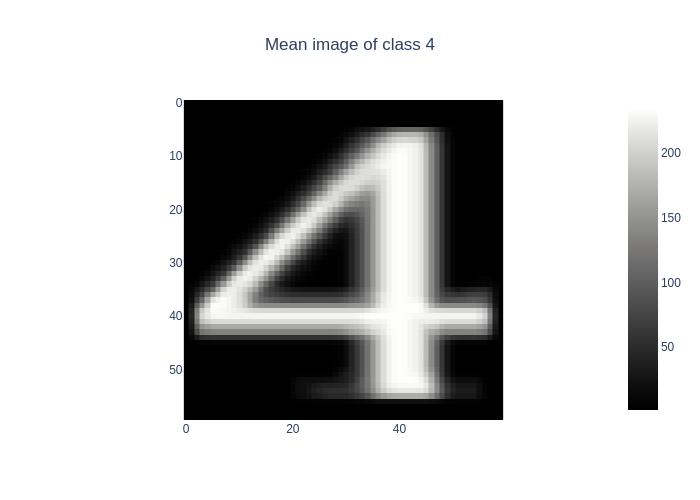
\includegraphics[width=\linewidth]{images/q2/partd/4_prototype.png}
    \end{subfigure}
    \hfill
    \begin{subfigure}{.3\linewidth}
        \centering
        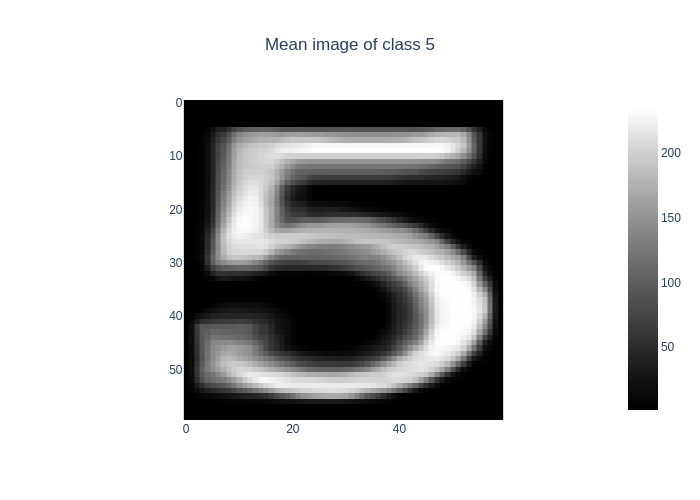
\includegraphics[width=\linewidth]{images/q2/partd/5_prototype.png}
    \end{subfigure}
    \newline
    \begin{subfigure}{.3\linewidth}
        \centering
        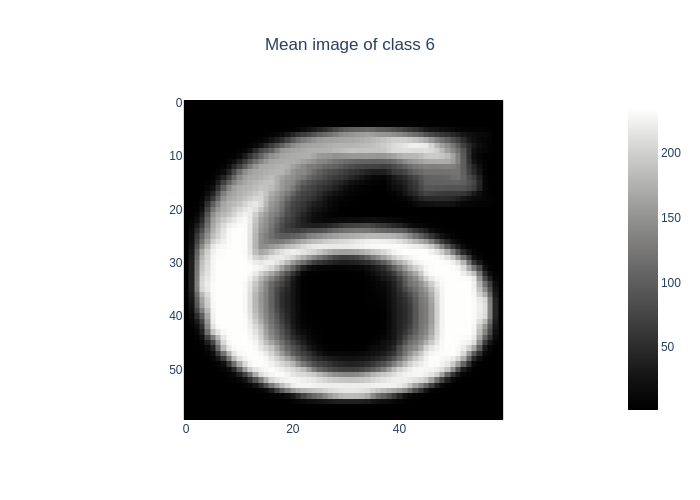
\includegraphics[width=\linewidth]{images/q2/partd/6_prototype.png}
    \end{subfigure}
    \hfill
    \begin{subfigure}{.3\linewidth}
        \centering
        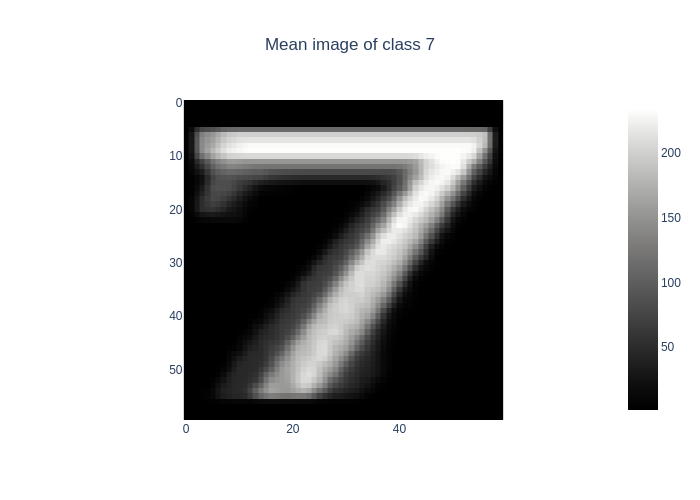
\includegraphics[width=\linewidth]{images/q2/partd/7_prototype.png}
    \end{subfigure}
    \hfill
    \begin{subfigure}{.3\linewidth}
        \centering
        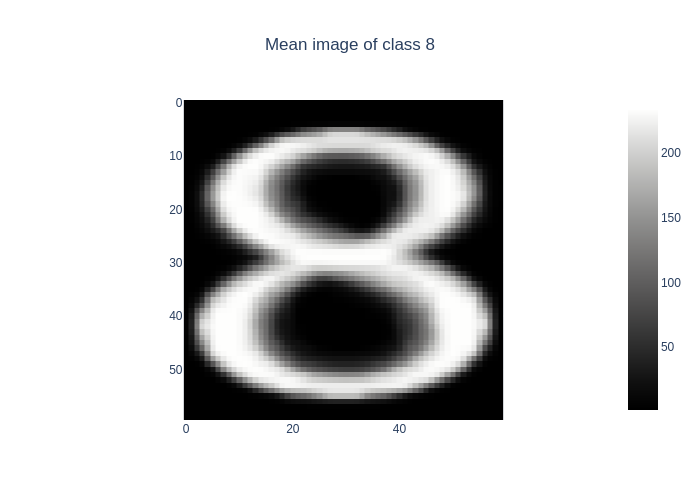
\includegraphics[width=\linewidth]{images/q2/partd/8_prototype.png}
    \end{subfigure}
    \newline
    \hfill
    \begin{subfigure}{.3\linewidth}
        \centering
        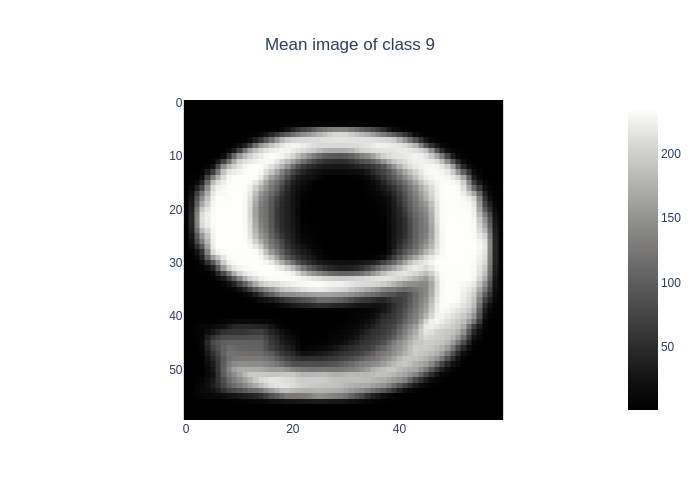
\includegraphics[width=\linewidth]{images/q2/partd/9_prototype.png}
    \end{subfigure}
    \hfill
    \caption{شکل میانگین متناظر هر یک از برچسب‌ها}
    \label{q2-partd}
\end{figure}

\newpage

\subsection*{قسمت ه}

با اضافه کردن داده‌های جدید انتظار داشتیم نتایج بیشتر افت کند اما نتایج حاصل شده نشان داد
که اضافه کردن داده‌های جدید تاثیر چندانی در افت دقت ندارد. با توجه به نتایج می‌توان بیان کرد که
الگوریتم \lr{MDC} در این مسئله بسیار خوب عمل کرده است چرا که حتی در هنگام دسته‌بندی تمامی داده‌ها
همچنان توانست دقت خوبی را ارائه دهد.

\newpage

\section*{سوال سه}

\subsection*{قسمت الف}

داریم.

$$P(Y_1, ..., Y_n|\lambda) = P(Y_1|\lambda)P(Y_2|\lambda)...P(Y_n|\lambda) = \prod_{i=1}^{s} P(Y_i|\lambda) = \prod_{i=1}^{s} \frac{(n_ix_i\lambda)^{y_i}e^{-n_ix_i\lambda}}{y_i!}$$

در عبارت بالا با توجه به مفهوم $k$ که تعداد دفعات رخداد یک پیشامد است، $k$ را با $y_i$ جایگزین کردیم.

\subsection*{قسمت ب}

خواهیم داشت.

\begin{eqnarray*}
    \hat{\lambda} & = & \text{argmax}\Big(\ln(P(Y_1, ..., Y_n|\lambda))\Big) \\
    & = & \sum_{i=1}^{s} \ln\Big(\frac{(n_ix_i\lambda)^{y_i}e^{-n_ix_i\lambda}}{y_i!}\Big) \\
    & = & \sum_{i=1}^{s} \ln\big((n_ix_i\lambda)^{y_i}e^{-n_ix_i\lambda}\big) - \ln y_i! \\
    & = & \sum_{i=1}^{s} \Big( \ln(n_ix_i\lambda)^{y_i} + \ln (e^{-n_ix_i\lambda}) - \ln y_i! \Big)\\
    & = & \sum_{i=1}^{s} \Big( y_i \times \ln(n_ix_i\lambda) - n_ix_i\lambda - \ln y_i! \Big) \\
\end{eqnarray*}

حال از عبارت بالا نسبت به $\lambda$ مشتق می‌گیریم.

\begin{eqnarray*}
    \frac{d}{d \lambda}(\sum_{i=1}^{s} \Big( y_i \times \ln(n_ix_i\lambda) - n_ix_i\lambda - \ln y_i! \Big)) & = & 0\\
    \sum_{i=1}^{s} \Big( \frac{y_i}{\lambda} - n_ix_i \Big) & = &  0\\
    \frac{1}{\lambda} \sum_{i=1}^{s} y_i - \sum_{i=1}^{s} n_ix_i & = & 0 \\
    \lambda & = & \frac{\sum_{i=1}^{s} y_i}{\sum_{i=1}^{s} n_ix_i} \\
\end{eqnarray*}

\subsection*{قسمت ج}

باید اثبات کنیم $E[\hat{\lambda}] = \lambda$. داریم.

\begin{eqnarray*}
    E[\hat{\lambda}] & = & \frac{1}{n} \sum_{j=1}^{n} \frac{\sum_{i=1}^{s} y_i}{\sum_{i=1}^{s} n_ix_i} \\
    & = & \frac{1}{n} \sum_{j=1}^{n} \frac{\sum_{i=1}^{s} n_ix_i \lambda}{\sum_{i=1}^{s} n_ix_i} \\
    & = & \frac{1}{n} \sum_{j=1}^{n} \lambda \frac{\sum_{i=1}^{s} n_ix_i }{\sum_{i=1}^{s} n_ix_i} \\
    & = & \frac{1}{n} \sum_{j=1}^{n} \lambda  = \lambda \\
\end{eqnarray*}

\subsection*{قسمت د}

داریم.

\begin{eqnarray*}
    E[(\hat{\lambda} - \lambda)^2] & = & E[\hat{\lambda}^2] - E[2\hat{\lambda}\lambda] + E[\lambda^2]\\
\end{eqnarray*}

حال سعی می‌کنیم تک‌تک عبارت‌های بالا را ساده‌تر کنیم.
\newline
برای $E[\hat{\lambda}^2]$ داریم.

\begin{eqnarray*}
    E[\hat{\lambda}] & = & E[\hat{\lambda}^2] - E^2[\hat{\lambda}] \\
    E[\hat{\lambda}^2] & = & \lambda + \lambda^2
\end{eqnarray*}

برای $E[2\hat{\lambda}\lambda]$ داریم.

\begin{eqnarray*}
    E[2\hat{\lambda}\lambda]  & = & 2\lambda E[\hat{\lambda}] \\
    & = & 2\lambda^2
\end{eqnarray*}

برای $E[\lambda^2]$ داریم.

\begin{eqnarray*}
    E[\lambda^2]  & = & E[(\frac{\sum_{i=1}^{s} y_i}{\sum_{i=1}^{s} n_ix_i})^2] \\
    & = & E[(\frac{\sum_{i=1}^{s} \lambda n_ix_i}{\sum_{i=1}^{s} n_ix_i})^2] \\
    & = & E[\lambda^2] \\
\end{eqnarray*}

\subsection*{قسمت ه}

باید مقدار $E[(\lambda -\hat{\lambda})^2]$ را محاسبه کنیم با توجه به مطالب اسلاید‌ها داریم.

$$E[(\lambda -\hat{\lambda})^2] = var(\hat{\lambda}) + (E[\hat{\lambda}] - \lambda)^2$$

با توجه به این که مقادیر واریانس و میانگین $\hat{\lambda}$ را در قسمت‌های قبلی محاسبه کردیم، بنابراین
این مقادیر را صرفا جایگذاری می‌کنیم.

$$E[(\lambda -\hat{\lambda})^2] = var(\hat{\lambda}) + 0 $$

\subsection*{قسمت و}

خواهیم داشت.

\begin{eqnarray*}
    \lambda & = & \frac{\sum_{i=1}^{s} y_i}{\sum_{i=1}^{s} n_ix_i} \\
    \lambda & = & \frac{2 + 5 + 14}{20 \times 0.4 + 50 \times 0.3 + 100 \times 0.6} = \frac{21}{83}
\end{eqnarray*}

\subsection*{قسمت ز}

خواهیم داشت.

\begin{eqnarray*}
    \hat{\lambda} & = & \text{argmax}\Big(\ln(P(Y_1, ..., Y_n|\lambda) P(\lambda))\Big) \\
    & = & \ln P(Y_1, ..., Y_n|\lambda) + \ln P(\lambda) \\
    & = & \ln P(Y_1, ..., Y_n|\lambda) + \ln \Big(\frac{\beta^\alpha}{\Gamma(\alpha)}\lambda^{\alpha-1} e^{-\beta \lambda}\Big) \\
    & = & \ln P(Y_1, ..., Y_n|\lambda) + \ln \frac{\beta^\alpha}{\Gamma(\alpha)} + (\alpha - 1)\ln \lambda - \beta \lambda \\
    & = & \sum_{i=1}^{s} \Big( y_i \times \ln(n_ix_i\lambda) - n_ix_i\lambda - \ln y_i! \Big)+ \ln \frac{\beta^\alpha}{\Gamma(\alpha)} + (\alpha - 1)\ln \lambda - \beta \lambda \\
\end{eqnarray*}

از عبارت بالا مشتق گرفته و مساوی صفر قرار می‌دهیم.

\begin{eqnarray*}
    \frac{d}{d\lambda}\Big(\sum_{i=1}^{s} \Big( y_i \times \ln(n_ix_i\lambda) - n_ix_i\lambda - \ln y_i! \Big)+ \ln \frac{\beta^\alpha}{\Gamma(\alpha)} + (\alpha - 1)\ln \lambda - \beta \lambda\Big) & = & 0 \\
    \sum_{i=1}^{s} \Big( \frac{y_i}{\lambda} - n_ix_i \Big) + \frac{a-1}{\lambda} - \beta & = & 0 \\
    \sum_{i=1}^{s} \frac{y_i}{\lambda} - \sum_{i=1}^{s}n_ix_i + \frac{\alpha-1}{\lambda} - \beta & = & 0 \\
    \lambda & = & \frac{(\alpha-1) + \sum_{i=1}^{s} y_i}{\beta + \sum_{i=1}^{s}n_ix_i} \\
\end{eqnarray*}

\section*{سوال چهار}

\subsection*{قسمت الف}

نمودار مربوط به تعداد رخداد هر یک از اعداد در شکل \ref{frequency-of-each-number} مشاهده می‌شود.

\begin{figure}[h]
    \centering
    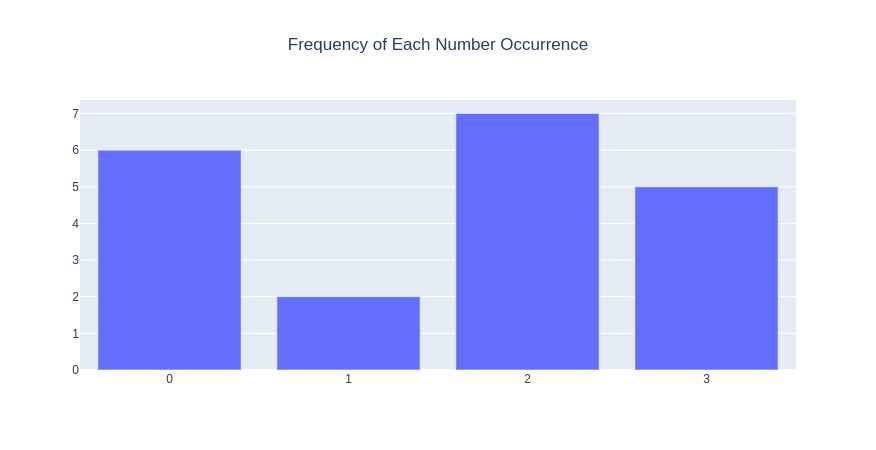
\includegraphics[scale=0.3]{images/q4/frequencies.png}
    \caption{تعداد رخداد هر یک از اعداد در مجموعه دادگان}
    \label{frequency-of-each-number}
\end{figure}

\subsection*{قسمت ب}

نمودار مربوط به احتمال رخداد هر یک از اعداد بر اساس دادگان دریافتی در شکل \ref{probability-of-each-number} مشاهده می‌شود.

\begin{figure}[h]
    \centering
    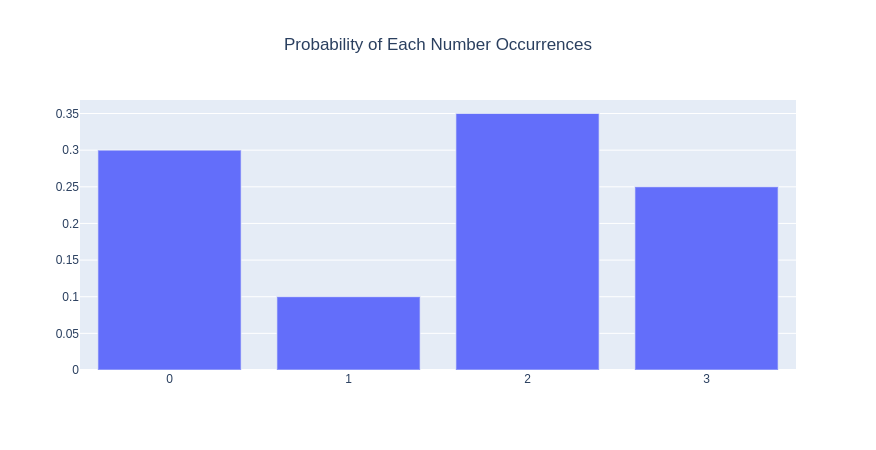
\includegraphics[scale=0.3]{images/q4/probability.png}
    \caption{احتمال رخداد هر یک از اعداد در مجموعه دادگان}
    \label{probability-of-each-number}
\end{figure}

\subsection*{قسمت ج}

نمودار تابع جرم احتمال متناظر هر یک از پارامتر‌های داده شده در شکل \ref{probability-mass-function} مشاهده می‌شود.

\begin{figure}[h]
    \centering
    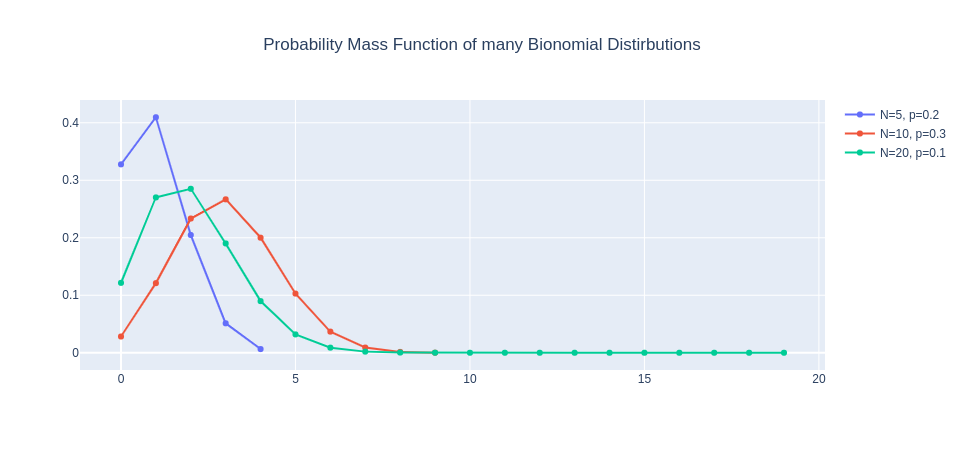
\includegraphics[scale=0.3]{images/q4/pmf.png}
    \caption{تابع جرم احتمال متناظر هر یک از پارامتر‌ها}
    \label{probability-mass-function}
\end{figure}

\subsection*{قسمت د}

در شکل \ref{probability-mass-function-compared-with-given-dataset} مقایسه‌ی
تابع جرم احتمال هر یک توزیع‌های داده شده با نمودار توزیع احتمال مجموعه دادگان
داده شده مشاهده می‌شود. با توجه به شکل به نظر می‌رسد که توزیع دوجمله‌ای با پارامتر‌های
$(N=20,p=0.1)$ بیشترین هماهنگی را با مجموعه دادگان داده شده دارد.

\begin{figure}[h]
    \centering
    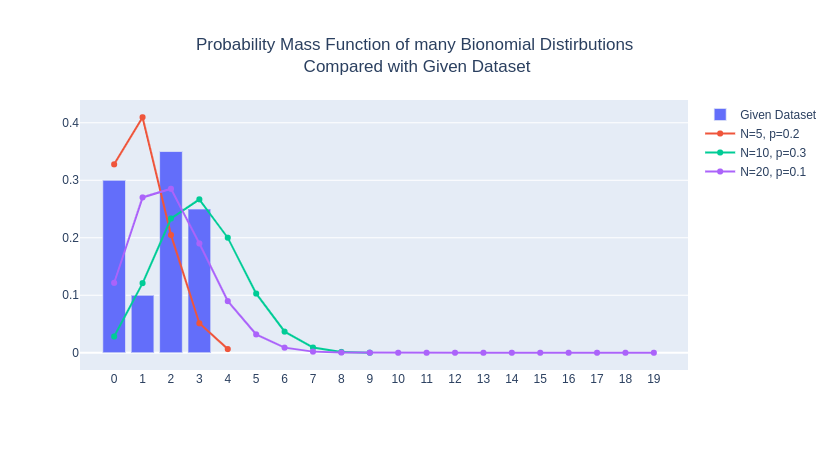
\includegraphics[scale=0.3]{images/q4/pmf_compared_with_dataset.png}
    \caption{مقایسه توزیع جرم احتمال متناظر هر یک از پارامتر‌های داده شده با مجموعه دادگان}
    \label{probability-mass-function-compared-with-given-dataset}
\end{figure}

\subsection*{قسمت ه}

در شکل \ref{likelihood} شکل تابع \lr{Likelihood} به ازای مقادیر مختلف $N$ رسم شده است. همان‌طور
که مشاهده می‌شود این تابع به ازای $N=8$ به ماکسیمم خود می‌رسد. بنابراین بهترین تصمیم برای
پارامتر $N$ مقدار $8$ است.

\begin{figure}[h]
    \centering
    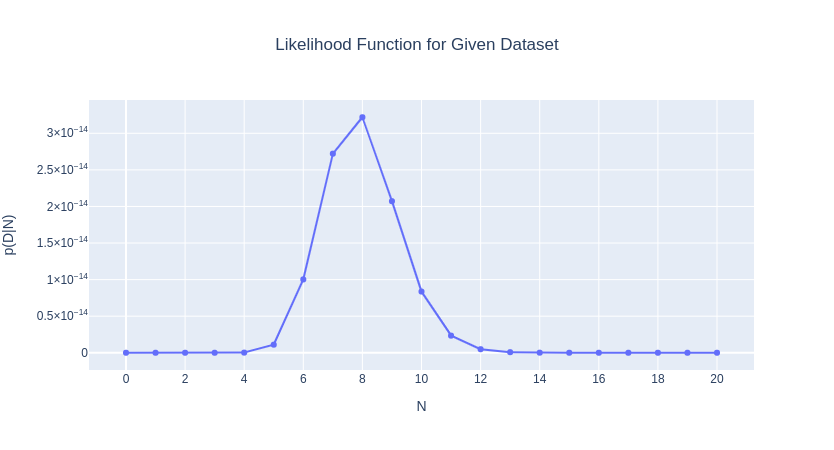
\includegraphics[scale=0.3]{images/q4/likelihood.png}
    \caption{تابع \lr{Likelihood} متناظر قسمت ه سوال چهار}
    \label{likelihood}
\end{figure}

\subsection*{قسمت و}

در شکل \ref{log-likelihood} شکل لگاریتم تابع \lr{Likelihood} به ازای مقادیر مختلف $N$ رسم شده است.
این شکل نیز ما را به نتیجه مشابهی در قبال $N$ می‌رساند.

\begin{figure}[h]
    \centering
    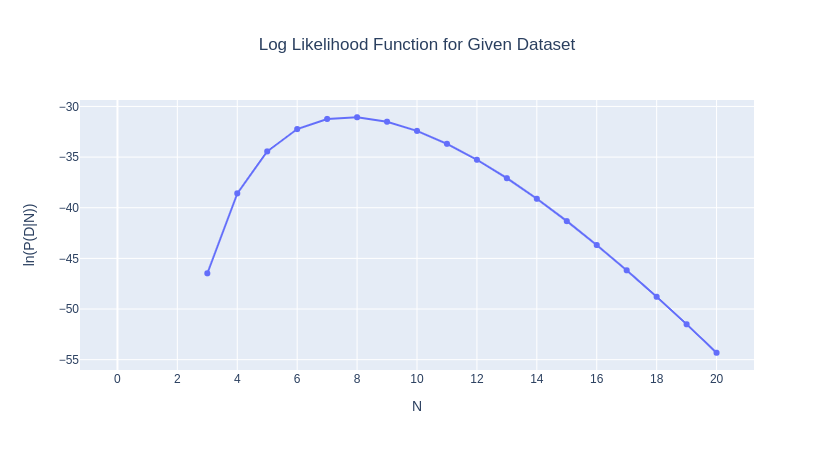
\includegraphics[scale=0.3]{images/q4/log_likelihood.png}
    \caption{تابع \lr{Likelihood} متناظر قسمت و سوال چهار}
    \label{log-likelihood}
\end{figure}

\subsection*{قسمت ز}

با توجه به شکل‌های \ref{likelihood} و \ref{log-likelihood} بهترین مقدار برای $N$ برابر $8$ است.

\subsection*{قسمت ح}

نمودار هیستوگرام مجموعه دادگان داده شده در شکل \ref{kumasarawamy} رسم شده است.

\begin{figure}[h]
    \centering
    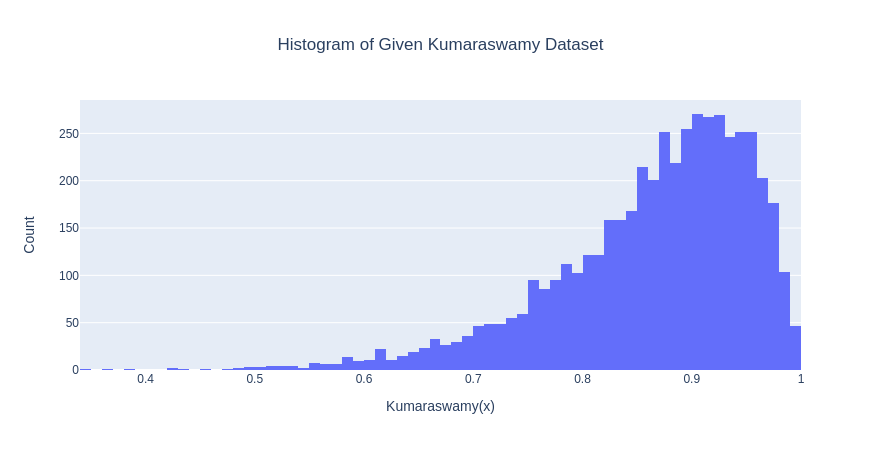
\includegraphics[scale=0.3]{images/q4/kumasarawamy.png}
    \caption{نمودار هیستوگرام مجموعه دادگان داده شده}
    \label{kumasarawamy}
\end{figure}

\subsection*{قسمت ط}

روابط \lr{Likelihood} و لگاریتم \lr{Likelihood} با فرض $\theta = (a, b)$ در ادامه آورده شده است.

\begin{eqnarray*}
    P(D|\theta) = \text{\lr{argmax}}(\prod_{i=1}^{n}p(x_i|\theta)) = \text{\lr{argmax}}(\prod_{i=1}^{n} abx_i^{a-1}(1-x_i^{a})^{b-1}) \\
\end{eqnarray*}
\begin{latin}
\begin{eqnarray*}
    \ln(P(D|\theta)) & = & \text{\lr{argmax}}(\ln(\prod_{i=1}^{n} abx_i^{a-1}(1-x_i^{a})^{b-1})) \\
    & = & \text{\lr{argmax}}(\sum_{i=1}^{n} \ln(abx_i^{a-1}(1-x_i^{a})^{b-1})) \\
    & = & \text{\lr{argmax}}(\sum_{i=1}^{n} \big( \ln(ab) + \ln(x_i^{a-1}) + \ln((1-x_i^{a})^{b-1}) \big) \\
    & = & \text{\lr{argmax}}(\sum_{i=1}^{n} \big( \ln(ab) + \ln(x_i^{a-1}) + \ln((1-x_i^{a})^{b-1}) \big) \\
    & = & \text{\lr{argmax}}(n\ln(ab) + (a-1) \sum_{i=1}^{n} \ln(x_i) + (b-1) \sum_{i=1}^{n} \ln(1-x_i^{a}))
\end{eqnarray*}
\end{latin}

\subsection*{قسمت ی}

با تغییر هر یک از مقادیر $a$ و $b$ در بازه $[0,12]$ و محاسبه مقدار تابع \lr{likelihood} متوجه می‌شویم که
بهترین مقدار برای $a=10$ و برای $b=2$ است.

\subsection*{قسمت ک}

برای این کار از تابع \lr{\texttt{differential\_evolution}} که توسط کتابخانه \lr{scipy} توسعه یافته استفاده
می‌کنیم. از آن جا که بر اساس مستندات کتابخانه \lr{scipy} تابع \lr{\texttt{differential\_evolution}} همواره
کمینه تابع داده شده را محاسبه می‌کند بنابراین منفی عبارت زیر را به تابع می‌دهیم تا بدین طریق ماکسیمم
رابطه زیر حاصل شود. این رابطه پیش‌تر در قسمت «ط» همین سوال به دست آمده است.

$$\text{\lr{argmax}}(n\ln(ab) + (a-1) \sum_{i=1}^{n} \ln(x_i) + (b-1) \sum_{i=1}^{n} \ln(1-x_i^{a}))$$

این تابع برای $a=9.753$ و $b=2.017$ را پیش‌بینی می‌کند. البته لازم به ذکر است که با توجه به \lr{stochastic}بودن
الگوریتم استفاده شده در تابع \lr{\texttt{differential\_evolution}} با اجرای مکرر،
نتایج هر بار اندکی تفاوت می‌کند.

\subsection*{قسمت ل}

حاصل مقادیر پیش‌بینی شده در قسمت‌های «ک» و «ی» در شکل \ref{comparison-stochastic-likelihood} دیده می‌شود.
همان‌طور که مشاهده می‌شود از آن جا که پارامتر تولید شده توسط هر دو روش به یکدیگر نزدیک است،
بنابراین مطابق انتظار نمودار تولید شده توسط هر دو روش مشابه یکدیگر است.

\begin{figure}[h]
    \centering
    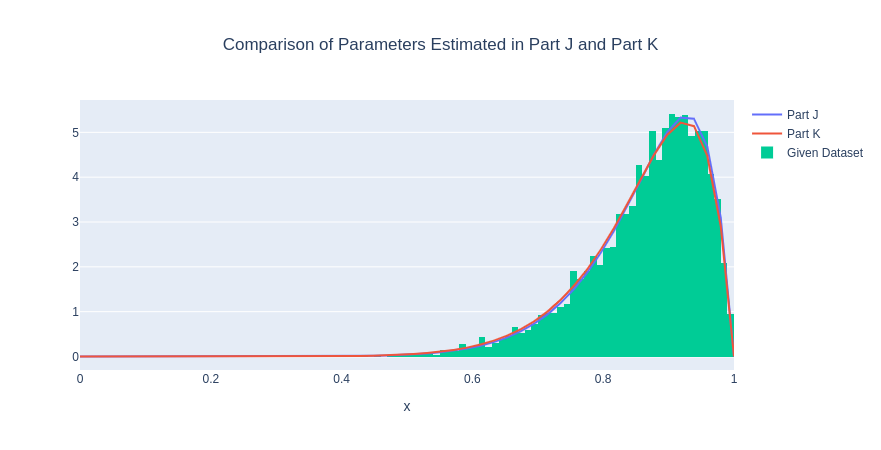
\includegraphics[scale=0.3]{images/q4/comparison_stochastic_likelihood.png}
    \caption{مقایسه نمودار حاصل شده با روش \lr{likelihood} و \lr{stochastic}}
    \label{comparison-stochastic-likelihood}
\end{figure}

\section*{سوال پنج}

\subsection*{قسمت الف و ب}

در این قسمت با توجه به آن که اکثرا هنگامی که یک نمونه $10$تایی از داده‌ها انتخاب می‌کردیم در محاسبه‌ی
تابع توزیع نرمال چندجمله‌ای به خطای \lr{Sigular Matrix} برمی‌خوردیم در نتیجه سوال را با نمونه‌های
$20$ و $50$ و $100$تایی انجام دادیم.

با انجام دسته‌بندی با استفاده از نمونه‌های $20$، $50$ و $100$تایی از داده‌ها نرخ خطا به ترتیب برابر
$0.405$، $0.255$ و $0.31$ می‌شود.

\subsection*{قسمت ج}

با انجام دسته‌بندی با استفاده از نمونه‌های $20$، $50$ و $100$تایی از داده‌ها نرخ خطا به ترتیب برابر
$0.32$، $0.27$ و $0.305$ می‌شود. همان‌طور که مشاهده می‌شود، نتایج نسبت به حالت قبلی اندکی بهتر شده است که دلیل آن را می‌توان
در دخیل کردن احتمال‌های اولیه در محاسبه‌ی احتمال دانست.

\subsection*{قسمت د}

بر مبنای محاسبات انجام شده کم‌ترین خطا در هنگام دسته‌بندی با استفاده از دو ویژگی، هنگامی رخ می‌دهد که
از ویژگی‌های \lr{mcv} و \lr{sgpt} استفاده کنیم. مرز تصمیم دسته‌بندی بیز حاصل شده با استفاده از این دو ویژگی در
شکل \ref{bayes-decision-boundary} رسم شده است.

\begin{figure}[h]
    \centering
    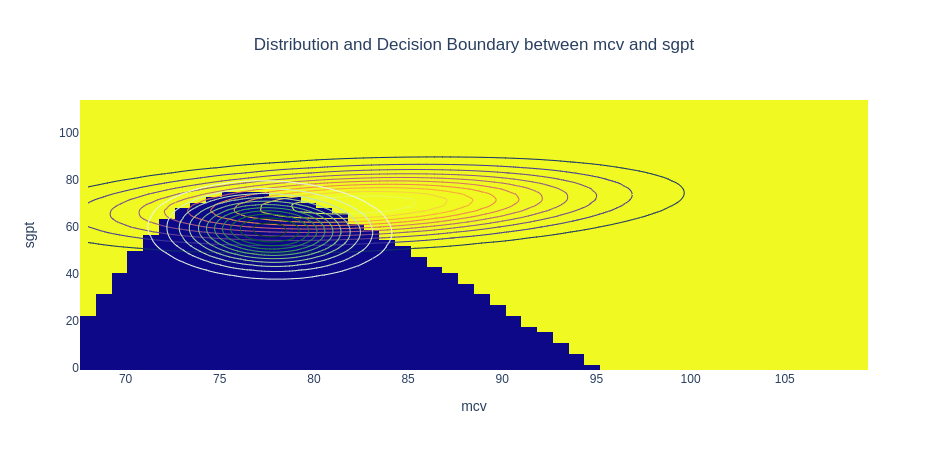
\includegraphics[scale=0.3]{images/q5/bayes_decision.png}
    \caption{مرز تصمیم بیز در قسمت د سوال پنج، قسمت زرد ناحیه متناظر با افراد معتاد است.}
    \label{bayes-decision-boundary}
\end{figure}

\subsection*{قسمت ه}

با فرض آن که کلاس $1$ متناظر داده‌های معتاد باشد و کلاس $2$ متناظر داده‌های کلاس غیرمعتاد باشد،
شکل دسته‌بند با در نظرگرفتن $\lambda$های داده به شکل \ref{bayes-decision-lambda-boundary} می‌شود.

\begin{figure}[h]
    \centering
    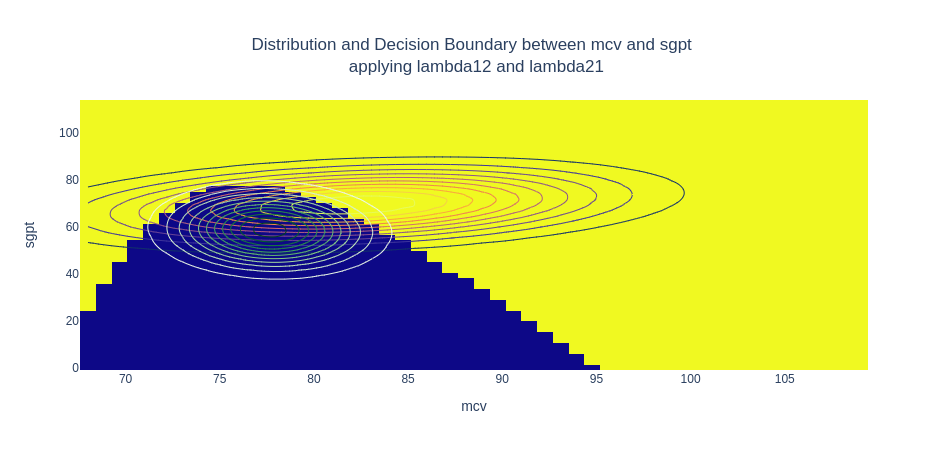
\includegraphics[scale=0.3]{images/q5/bayes_decision_lambda.png}
    \caption{مرز تصمیم بیز در قسمت ه سوال پنج، قسمت زرد ناحیه متناظر با افراد معتاد است.}
    \label{bayes-decision-lambda-boundary}
\end{figure}

\section*{سوال شش}

\subsection*{قسمت الف}

با اندازه‌گیری احتمال‌ها به شرح زیر به دست می‌آید.

$$P(\text{\lr{skin}}) = 0.7249 \hspace{1cm} P(\text{\lr{not skin}}) = 0.2750$$

\subsection*{قسمت ب}

میانگین و کواریانس متناظر هر دسته در جدول \ref{skin-non-skin-mean-covariance} آورده شده است.

\begin{table}[h]
    \centering
    \caption{میانگین و کواریانس متناظر کلاس‌های پوست و غیر‌پوست}
    \label{skin-non-skin-mean-covariance}
    \begin{tabular}{c|c|c}
        & میانگین & کواریانس \\
        \hline
        & & \\
        پوست & $\begin{bmatrix} 111.69\\ 140.48\\ 189.93 \end{bmatrix}$ & $\begin{bmatrix} 2675.40 & 2449.30 & 1861.13 \\ 2449.30 & 2383.49 & 1953.49 \\ 1861.13 & 1953.49 & 1962.10 \end{bmatrix}$ \\
        & & \\
        غیرپوست & $\begin{bmatrix}96.43 \\ 106.52 \\ 129.37 \end{bmatrix}$ & $\begin{bmatrix}7145.14 & 6916.65 & 6294.89 \\ 6916.65 & 7075.67 & 6717.72 \\ 6294.89 & 6717.72 & 7762.24 \end{bmatrix}$
    \end{tabular}
\end{table}

\subsection*{قسمت ج}

دسته‌بندی به نحو موجود در شکل \ref{partc-trump-skin} انجام می‌شود.

\begin{figure}[h]
    \begin{subfigure}{.45\linewidth}
        \centering
        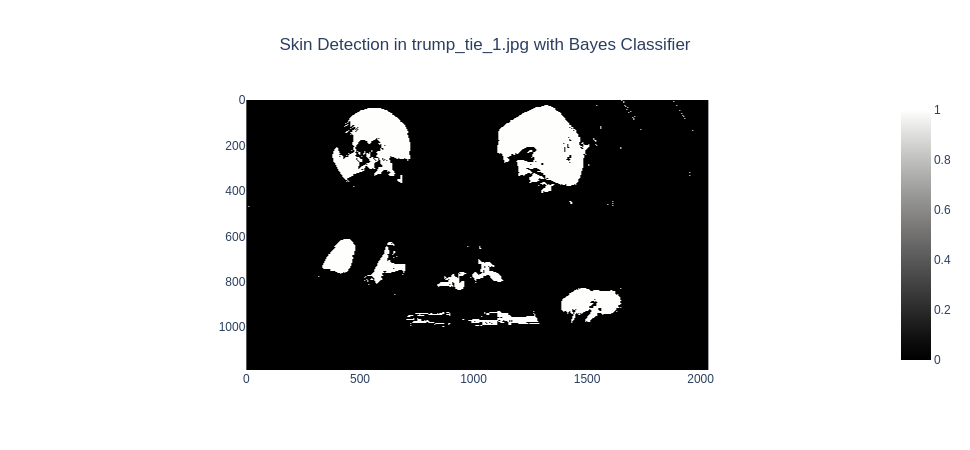
\includegraphics[width=\linewidth]{images/q6/trump_partc.png}
    \end{subfigure}
    \hfill
    \begin{subfigure}{.45\linewidth}
        \centering
        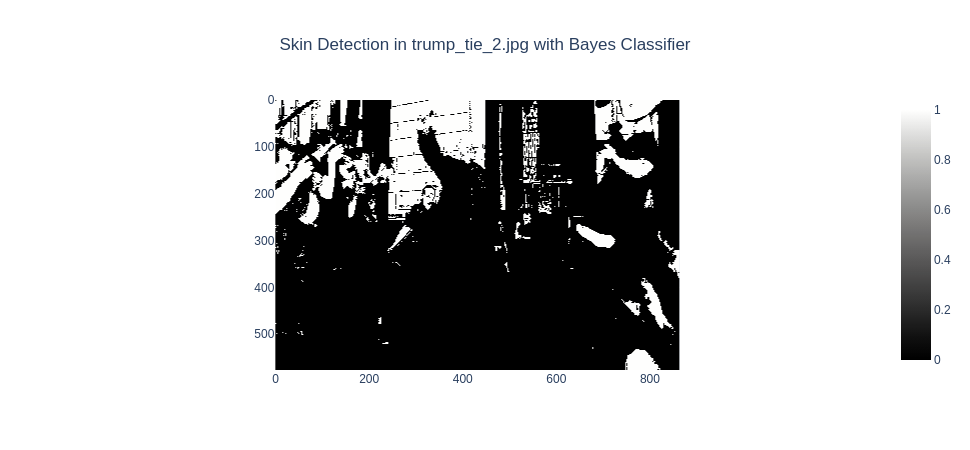
\includegraphics[width=\linewidth]{images/q6/trump_partc2.png}
    \end{subfigure}
    \caption{پیش‌بینی مدل بیز برای تصاویر ترامپ، قسمت ج سوال ۶}
    \label{partc-trump-skin}
\end{figure}

\subsection*{قسمت د}

دسته‌بندی به نحو موجود در شکل \ref{partd-trump-skin} انجام می‌شود. دسته‌بندی انجام شده توسط دسته‌بند \lr{MDC}
دقت کمتری نسبت به دسته‌بند بیز دارد. البته دسته‌بند بیز نیز نمی‌تواند همه‌ی داده‌های پوست را تشخیص دهد، برای مثال در
شکل \lr{trump\_tie\_2.jpg} پای یکی از خبرنگاران سیاه‌پوست اصلا تشخیص داده نشده است. علت این که دقت دسته‌بندی
انجام شده توسط \lr{MDC} از بیز کم‌تر است آن است که دسته‌بند \lr{MDC} تنها به فاصله اقلیدسی توجه دارد در صورتی که
دسته‌بند \lr{Bayes} علاوه بر فاصله به توزیع داده‌ها نیز توجه می‌کند.

\begin{figure}[h]
    \begin{subfigure}{.45\linewidth}
        \centering
        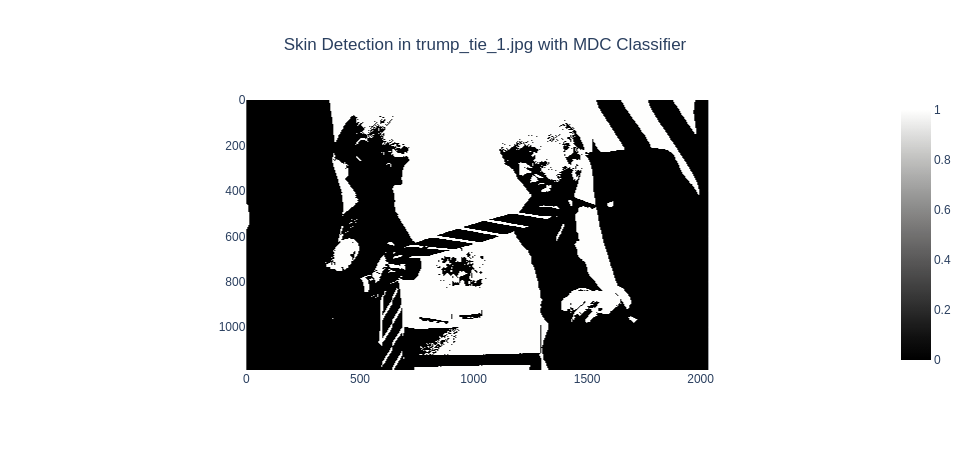
\includegraphics[width=\linewidth]{images/q6/trump_partd.png}
    \end{subfigure}
    \hfill
    \begin{subfigure}{.45\linewidth}
        \centering
        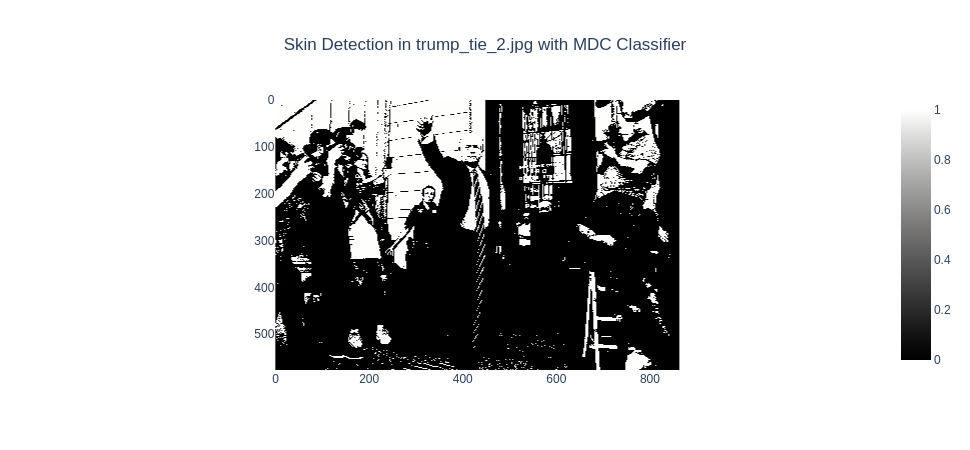
\includegraphics[width=\linewidth]{images/q6/trump_partd2.png}
    \end{subfigure}
    \caption{پیش‌بینی مدل \lr{MDC} برای تصاویر ترامپ، قسمت د سوال ۶}
    \label{partd-trump-skin}
\end{figure}

\subsection*{قسمت ه}

با دسته‌بندی انجام شده توسط بیز نرخ خطا $21.89$ درصد است.

\subsection*{قسمت و}

ماتریس در‌هم‌ریختگی متناظر این مدل در جدول \ref{partf-confusion-matrix} آمده است.

\begin{table}[h]
    \centering
    \caption{ماتریس درهم‌ریختگی قسمت و سوال شش}
    \label{partf-confusion-matrix}
    \begin{tabular}{c|c|c}
        & غیر پوست & پوست \\
        \hline
        غیر پوست & $1747794$ & $541749$ \\
        پوست & $52292$ & $371343$
    \end{tabular}
\end{table}

\subsection*{قسمت ز}

محاسبه انتگرال متناظر این قسمت از دو جهت پیچیده است: (۱) انتگرال باید بر روی سه داده‌های سه متغیره محاسبه شود،
(۲) محاسبه‌ی خط جداکننده بین دو کلاس با توجه به چند متغیره بودن دشوار است و (۳) با توجه به محاسبات قبلی
کواریانس‌های متناظر دو توزیع برابر نیستند و در نتیجه جداکننده بین دو کلاس خطی نیست. با توجه به این دلایل از کتابخانه
\lr{\texttt{scipy.integrate.nquad}} برای محاسبه انتگرال کمک می‌گیریم. این انتگرال را در بازه $[0,255]$ برای
هر سه متغیر حساب می‌کنیم. اما از آن جا که محاسبه این انتگرال نیز بسیار طولانی است تنها در نقاط صحیح
مقدار انتگرال را محاسبه می‌کنیم. با محاسبه انتگرال تنها بر روی نقاط صحیح مقدار خطای \lr{Bayes} برابر
$9.84 \times 10^{-5}$ به دست می‌آید.

\subsection*{قسمت ح}

نمودار \lr{ROC} این دسته‌بند به شکل \ref{roc} حاصل می‌شود.

\begin{figure}[h]
    \centering
    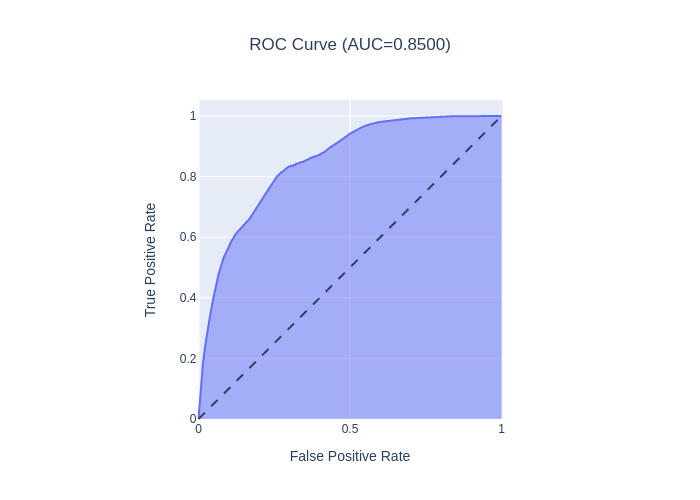
\includegraphics[scale=0.3]{images/q6/roc.png}
    \caption{نمودار \lr{ROC} متناظر دسته‌بند در قسمت ح سوال ۶}
    \label{roc}
\end{figure}

\subsection*{قسمت ط}


\subsubsection*{قسمت الف}

با اندازه‌گیری احتمال‌ها به شرح زیر به دست می‌آید.

$$P(\text{\lr{skin}}) = 0.8304 \hspace{1cm} P(\text{\lr{not skin}}) = 0.1695$$

\subsubsection*{قسمت ب}

میانگین و کواریانس متناظر هر دسته در جدول \ref{parti-skin-non-skin-mean-covariance} آورده شده است.

\begin{table}[h]
    \centering
    \caption{میانگین و کواریانس متناظر کلاس‌های پوست و غیر‌پوست}
    \label{parti-skin-non-skin-mean-covariance}
    \begin{tabular}{c|c|c}
        & میانگین & کواریانس \\
        \hline
        & & \\
        پوست & $\begin{bmatrix}103.72 \\ 126.67 \\ 173.68\end{bmatrix}$ & $\begin{bmatrix}2401.05 & 2305.46 & 2037.52 \\ 2305.46 & 2405.40 & 2283.40 \\ 2037.52 & 2283.40 & 2547.09 \end{bmatrix}$ \\
        & & \\
        غیرپوست & $\begin{bmatrix}97.25 \\ 103.54 \\ 118.23\end{bmatrix}$ & $\begin{bmatrix}5826.86 & 5463.83 & 4909.88 \\ 5463.83 & 5749.03 & 5366.70 \\ 4909.88 & 5366.70 & 6283.84 \\\end{bmatrix}$
    \end{tabular}
\end{table}

\subsubsection*{قسمت ج}

دسته‌بندی به نحو موجود در شکل \ref{parti-partc-trump-skin} انجام می‌شود. در این حالت به نظر می‌رسد که
دقت پیش‌بینی افت کرده و بعضی از قسمت‌هایی که پوست نیستند نیز به عنوان پوست تشخیص داده می‌شوند.

\begin{figure}[h]
    \begin{subfigure}{.45\linewidth}
        \centering
        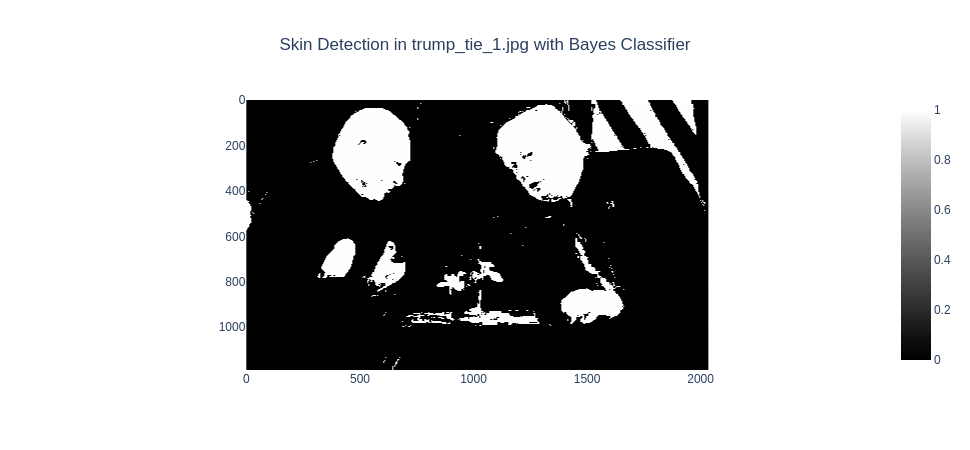
\includegraphics[width=\linewidth]{images/q6/parti_trump_partc.png}
    \end{subfigure}
    \hfill
    \begin{subfigure}{.45\linewidth}
        \centering
        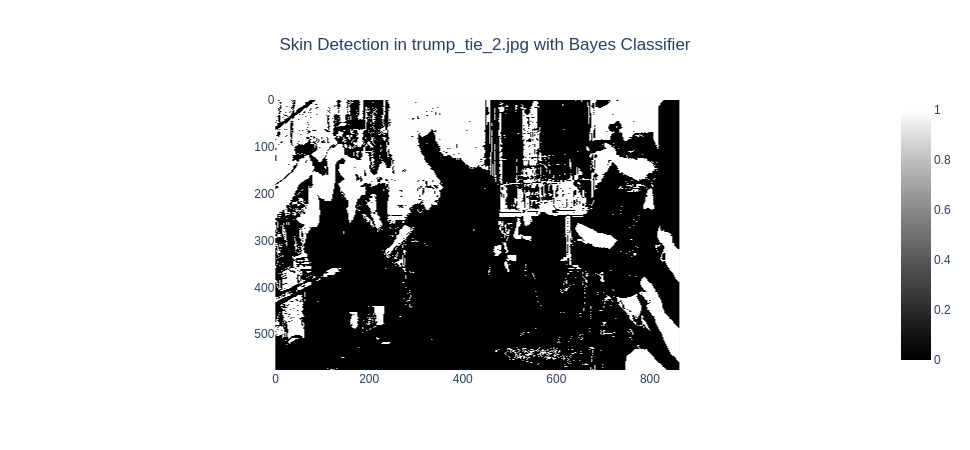
\includegraphics[width=\linewidth]{images/q6/parti_trump_partc2.png}
    \end{subfigure}
    \caption{پیش‌بینی مدل بیز برای تصاویر ترامپ، قسمت ط سوال ۶}
    \label{parti-partc-trump-skin}
\end{figure}

\subsubsection*{قسمت د}

دسته‌بندی به نحو موجود در شکل \ref{parti-partd-trump-skin} انجام می‌شود. تنایج متناظر این دسته‌بندی چندان تغییر نمی‌کند،
چرا که میانگین داده‌ها چندان تفاوتی نکرده است. اما همچنان نرخ خطای این دسته‌بند نسبت به دسته‌بند بیز کم‌تر است. برای مثال
دسته‌بند بیز در تصویر \lr{trump\_tie\_1.jpeg} دیوار را به درستی غیر پوست تشخیص داده است اما دسته‌بند \lr{MDC}
دیوار را به اشتباه پوست تشخیص داده است.

\begin{figure}[h]
    \begin{subfigure}{.45\linewidth}
        \centering
        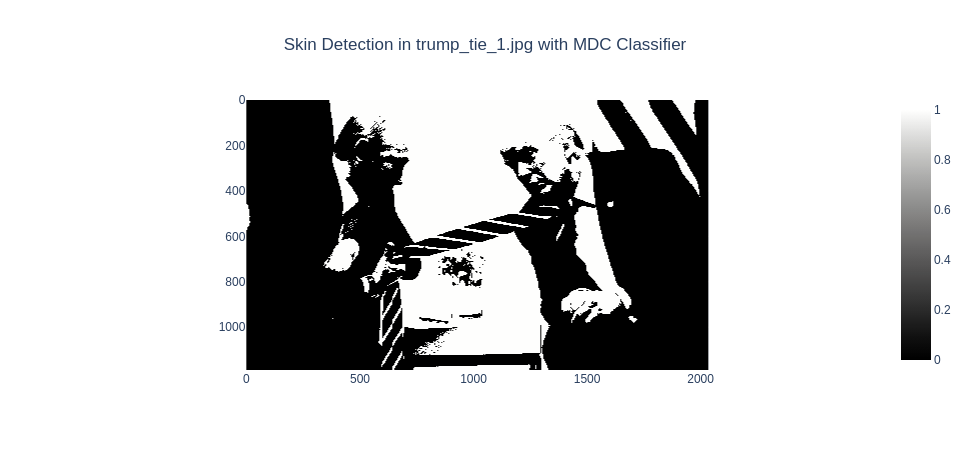
\includegraphics[width=\linewidth]{images/q6/parti_trump_partd.png}
    \end{subfigure}
    \hfill
    \begin{subfigure}{.45\linewidth}
        \centering
        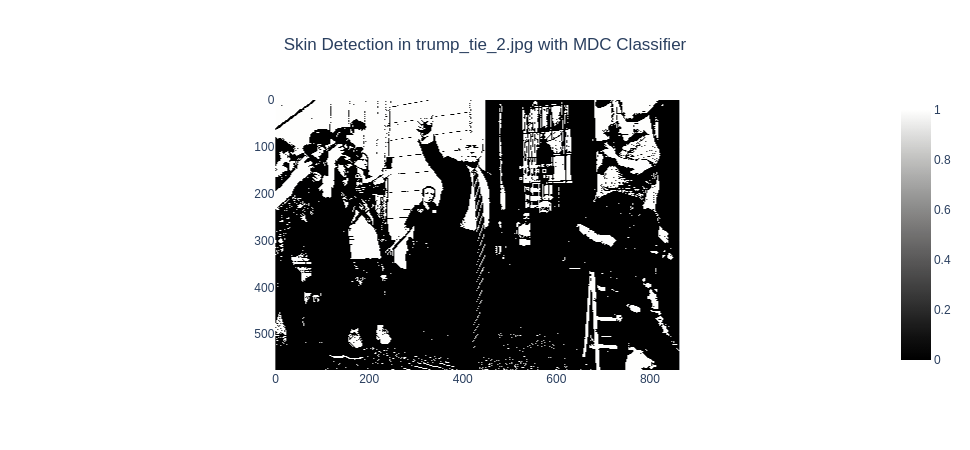
\includegraphics[width=\linewidth]{images/q6/parti_trump_partd2.png}
    \end{subfigure}
    \caption{پیش‌بینی مدل \lr{MDC} برای تصاویر ترامپ، قسمت ط سوال ۶}
    \label{parti-partd-trump-skin}
\end{figure}

\subsubsection*{قسمت ه}

با دسته‌بندی انجام شده توسط بیز نرخ خطا $40.69$ درصد است که نسبت به قبل حدود $20$ درصد بیشتر شده است.

\subsubsection*{قسمت و}

ماتریس در‌هم‌ریختگی متناظر این مدل در جدول \ref{parti-partf-confusion-matrix} آمده است.
با مقایسه این جدول با جدول قبلی مشاهده می‌شود که بسیاری از پیکسل‌هایی که معرف پوست نیستند در این حالت
به عنوان پیکسل پوست تشخیص داده می‌شوند که این امر موجب افت دقت شده است. این اتفاق را می‌توان این گونه توجیه کرد
که با افزایش داده‌های پوست مدل سعی کرده است رنگ‌های پوست بیشتری را تشخیص دهد ولی این اتفاق موجب شده است که
بعضی از قسمت‌هایی که پوست نیستند نیز پوست تشخیص داده شوند.

\begin{table}[h]
    \centering
    \caption{ماتریس درهم‌ریختگی قسمت و سوال شش}
    \label{parti-partf-confusion-matrix}
    \begin{tabular}{c|c|c}
        & غیر پوست & پوست \\
        \hline
        غیر پوست & $1209475$ & $1080068$ \\
        پوست & $24088$ & $399547$
    \end{tabular}
\end{table}

\subsubsection*{قسمت ز}

مشابه قسمت قبل مقدار خطا را محاسبه می‌کنیم که در این حالت مقدار انتگرال برابر $7.33 \times 10^{-5}$ به دست می‌آید.
در این قسمت بر خلاف انتظار حاصل انتگرال کاهش یافته است. کاهش انتگرال محاسبه شده را می‌توان به این شکل توجیه کرد که
با افزایش نمونه‌ها کواریانس داده‌های غیرپوست کاهش یافته است در نتیجه این کاهش کواریانس توزیع جمع‌تر شده که در نتیجه
حاصل این انتگرال شده کم‌تر است.

\subsubsection*{قسمت ح}

نمودار \lr{ROC} این دسته‌بند به شکل \ref{parti-roc} حاصل می‌شود. همان‌طور که در قسمت‌های قبلی دیدیم دقت مدل
کاهش یافته بود و در این شکل نیز مطابق انتظار ناحیه زیر نمودار در این شکل کاهش یافته است.

\begin{figure}[h]
    \centering
    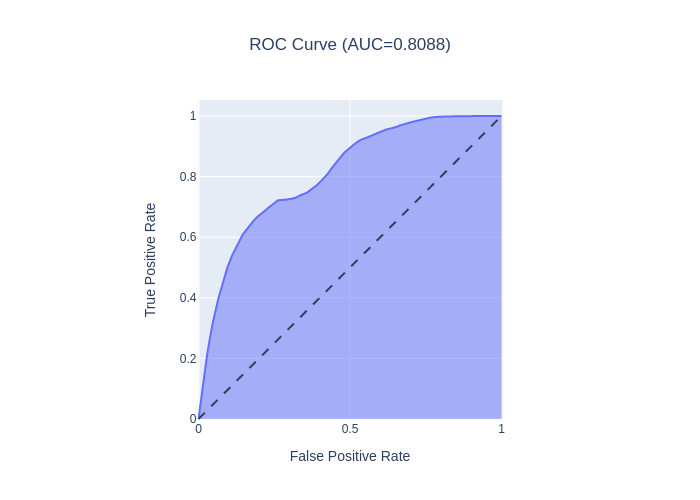
\includegraphics[scale=0.3]{images/q6/parti_roc.png}
    \caption{نمودار \lr{ROC} متناظر دسته‌بند در قسمت ح سوال ۶}
    \label{parti-roc}
\end{figure}

\section*{سوال هفت}

\subsection*{قسمت الف}

دسته‌بند بیز برای محاسبه مقدار احتمال $P(c_i|x)$ به مقادیر دو احتمال $P(c_i)$ و $P(x|c_i)$ نیاز دارد. محاسبه احتمال $P(c_i)$ شاید کار
ساده‌ای باشد اما محاسبه احتمال $P(x|c_i)$ دشوار بوده و نیاز به داده فراوانی دارد. چرا که باید مقدار احتمال
$x$ به ازای هر کلاس محاسبه شود. بنابراین مهم‌ترین نقطه ضعف این الگوریتم نیاز داشتن به داده فراوان است.
در ادامه برخی دیگر از معایب این الگوریتم را نیز برمی‌شماریم.

\begin{itemize}
    \item این دسته‌بند همواره فرض می‌کند ویژگی‌های مختلف از هم مستقل هستند. این فرض از لحاظ تئوری درست است،
    اما در دنیای واقعی همیشه برقرار نیست.
    \item اگر برای یکی از کلاس‌ها رخدادی نداشته باشیم، این الگوریتم مقدار متناظر آن را صفر در می‌گیرد که منطقی نیست.
\end{itemize}

\subsection*{قسمت ب}

بله، انجام چنین کاری با استفاده از مدل گاوسی امکان‌پذیر است. در مسائل رگرسیون معمولا به دنبال تابعی خطی هستیم
که رابطه‌ی بین بردار ورودی $x$ و خروجی $y$ را بیان کند،به عبارتی به دنبال $\theta$ای هستیم که

$$y = \theta^T x + \epsilon $$

باشد. در عبارت بالا منظور از $\epsilon$ خطای خطی سازی است و ما فرض می‌کنیم که این خطا دارای توزیع
$\mathcal{N} (0, \sigma^2)$ است. بنابراین خواهیم داشت.

$$y \sim \mathcal{N}(\theta^T x, \sigma^2)$$

با اندکی دقت در رابطه‌ی بالا متوجه می‌شویم که این مسئله یک مسئله تخمین پارامتر است و در نتیجه می‌توان با استفاده
از روش‌های \lr{Maximum Likelihood Estimation} و \lr{Bayesian Estimation} مقدار متناظر $\theta$ و $\sigma$ را
محاسبه کرد.

\subsection*{قسمت ج}

هر یک از معیار‌های فاصله مزایا و معایبی دارد. برای مثال در شکل \ref{euclidean-vs-mahalanobis} دو معیار فاصله
اقلیدسی و \lr{mahalanobis} مقایسه شده‌اند. در این شکل دایره نشانگر فاصله با طول $K$ با معیار فاصله اقلیدسی
و بیضی نشانگر فاصله $K$ای که با معیار فاصله \lr{mahalanobis} اندازه گرفته شده است، می‌باشد. همان‌طور که مشاهده
می‌شود معیار \lr{mahalanobis} از آن جا که به توزیع داده‌ها نیز اهمیت می‌دهد اگر برای تصمیم‌گیر \lr{Min Distance}
استفاده شود، در کلاس‌هایی که توزیع داده‌ها یکنواخت نیست می‌تواند نتیجه بهتری بگیرد.

\begin{figure}[h]
    \centering
    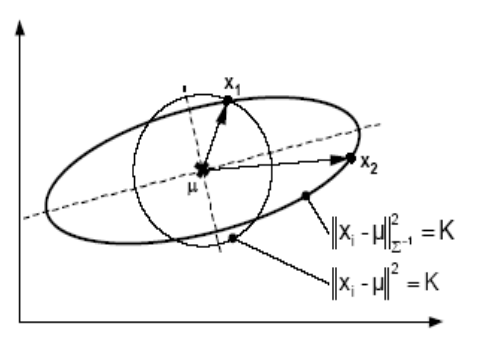
\includegraphics[scale=0.3]{images/q7/euclidean_vs_manhataan.png}
    \caption{مقایسه معیار‌های فاصله اقلیدسی و \lr{mahalanobis}}
    \label{euclidean-vs-mahalanobis}
\end{figure}

علاوه بر معیار فاصله \lr{mahalanobis}، معیار فاصله شباهت کسینوسی را نیز با فاصله اقلیدسی مقایسه می‌کنیم.
این معیار فاصله به صورت زیر بین دو بردار $v_1$ و $v_2$ تعریف می‌شود.

$$\text{\lr{cosine similarity}} = \frac{v_1.v_2}{|v_1||v_2|}$$

همان‌طور که مشاهده می‌شود این معیار فاصله زاویه‌ی بین دو بردار را به عنوان شباهت انتخاب کرده و بزرگی
بردار تاثیری در معیار فاصله ندارد. به عنوان مثال در شکل \ref{cosine-similarity}  فاصله‌ی بین بردار‌های
$x_1$ از $x_2$ برابر با فاصله $d_1$ و $d_2$ است. همچنین بر اساس این معیار، فاصله بین $x_1$ و $d_1$
برابر صفر است.

\begin{figure}[h]
    \centering
    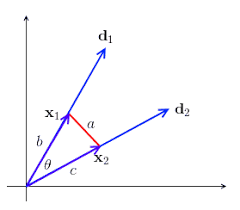
\includegraphics[scale=0.3]{images/q7/cosine.png}
    \caption{معیار‌های فاصله شباهت کسینوسی}
    \label{cosine-similarity}
\end{figure}

\subsection*{قسمت د}

در دسته‌بند بیز در هنگام آموزش باید مقادیر احتمال‌های $P(\omega_i)$ و $P(x|\omega_i)$ باید محاسبه شود.
در \lr{MDC} نیز در مرحله‌ آموزش میانگین متناظر هر یک از کلاس‌ها محاسبه شده و در مرحله‌ی تست فاصله‌ی
داده‌ی دریافتی از هر یک از این مراکز دسته‌ها محاسبه می‌شود. برای داده جدید، برچسب دسته‌ای که مرکز آن کمترین فاصله
را با داده جدید دارد نسبت داده می شود.

\subsection*{قسمت ه}

روش \lr{MAP} از احتمال‌های اولیه برای به دست آوردن احتمال توزیع پارامتر کمک می‌گیرد. حال اگر این احتمال‌های
اولیه دقیق نباشند در این صورت تخمینی که با استفاده از روش \lr{MAP} محاسبه می‌شود نسبت به روش \lr{MLE}
که تنها از احتمال \lr{Likelihood} کمک می‌گیرد ضعیف‌تر خواهد بود.

\end{document}